\documentclass[UTF8,10pt,landscape]{ctexart}

% Build with: xelatex cheatsheet-template.tex
% Or:         lualatex cheatsheet-template.tex

\usepackage[
  a4paper,
  landscape,
  left=6mm,
  right=6mm,
  top=6mm,
  bottom=6mm
]{geometry}
\usepackage{multicol}
\usepackage{amsmath,amssymb,mathtools}
\usepackage{booktabs,tabularx,array}
\usepackage[table]{xcolor}
\usepackage{graphicx}
\usepackage{listings}
\usepackage[hidelinks]{hyperref}

\definecolor{accent}{HTML}{0F766E}
\definecolor{accentlight}{HTML}{E6FFFA}
\definecolor{ink}{HTML}{111827}
\definecolor{muted}{HTML}{6B7280}
\definecolor{rulegray}{HTML}{D1D5DB}
\definecolor{codebg}{HTML}{F8FAFC}

\newcommand{\cheatbodyfont}{\fontsize{7.2pt}{7.7pt}\selectfont}
\newcommand{\cheatsectionfont}{\fontsize{8.2pt}{8.6pt}\selectfont}
\newcommand{\cheatsubsectionfont}{\fontsize{7.4pt}{7.8pt}\selectfont}
\newcommand{\cheattinyfont}{\fontsize{6.4pt}{6.8pt}\selectfont}

\pagestyle{empty}

\setlength{\parindent}{0pt}
\setlength{\parskip}{0.4pt}
\setlength{\columnsep}{3.2mm}
\setlength{\columnseprule}{0.15pt}
\setlength{\premulticols}{0pt}
\setlength{\postmulticols}{0pt}
\setlength{\multicolsep}{0pt}
\setlength{\tabcolsep}{2pt}
\setlength{\fboxsep}{1pt}
\renewcommand{\arraystretch}{0.82}

\makeatletter
\def\@listi{\leftmargin\leftmargini
  \topsep 0.4pt
  \parsep 0pt
  \partopsep 0pt
  \itemsep 0pt}
\let\@listI\@listi
\@listi
\makeatother

\newcommand{\cheatsection}[1]{%
  \vspace{3pt}%
  {\color{accent}\normalfont\bfseries\cheatsectionfont #1\par}%
  \vspace{-2.5pt}%
  {\color{accent}\rule{\linewidth}{0.3pt}\par}%
  \vspace{1pt}%
}
\newcommand{\cheatsubsection}[1]{%
  \vspace{1.6pt}%
  {\color{ink}\normalfont\bfseries\cheatsubsectionfont #1\par}%
  \vspace{0.2pt}%
}

\newcommand{\term}[1]{\textbf{\color{accent}#1}}
\newcommand{\key}[1]{\fcolorbox{rulegray}{accentlight}{\cheattinyfont\texttt{#1}}}
\newcommand{\code}[1]{\texttt{\cheatbodyfont #1}}
\newcommand{\note}[1]{%
  \begingroup
  \setlength{\fboxsep}{2pt}%
  \colorbox{accentlight}{%
    \parbox{\dimexpr\linewidth-2\fboxsep\relax}{\cheattinyfont #1}%
  }%
  \endgroup
}
\newenvironment{stemlist}{%
  \begingroup
  \cheattinyfont
  \setlength{\parskip}{0.6pt}%
}{%
  \par
  \endgroup
}
\newcommand{\stemrow}[2]{\par\noindent\term{#1}: #2\par}

\newcolumntype{Y}{>{\raggedright\arraybackslash}X}

\lstdefinestyle{cheatcode}{
  basicstyle=\ttfamily\cheattinyfont,
  backgroundcolor=\color{codebg},
  columns=fullflexible,
  keepspaces=true,
  breaklines=true,
  frame=single,
  rulecolor=\color{rulegray},
  framerule=0.2pt,
  xleftmargin=1pt,
  xrightmargin=1pt,
  aboveskip=1pt,
  belowskip=1pt
}
\lstset{style=cheatcode}

\begin{document}
\cheatbodyfont
\setlength{\abovedisplayskip}{1pt}
\setlength{\belowdisplayskip}{1pt}
\setlength{\abovedisplayshortskip}{0pt}
\setlength{\belowdisplayshortskip}{0pt}

\begin{multicols*}{5}
\cheatsection{1 Computer System Overview}
\cheatsubsection{Main Elements and Registers}
\begin{tabularx}{\linewidth}{@{}lY@{}}
\toprule
\term{Processor} & executes instructions and controls system operation.\\
\term{Main memory} & stores currently used programs and data.\\
\term{I/O modules} & move data between the computer and external devices.\\
\term{System bus} & carries data, address, and control signals among modules.\\
\bottomrule
\end{tabularx}
\term{User-visible registers}: referenced by machine instructions to reduce memory access.\\
\term{Control/status registers}: PC, IR, MAR, MBR, PSW; used by CPU and OS to control execution.

\cheatsubsection{Instruction Actions}
\begin{itemize}
  \item \term{Processor-memory}: load/store between CPU and memory.
  \item \term{Processor-I/O}: transfer data between CPU and I/O modules.
  \item \term{Data processing}: arithmetic or logical operations.
  \item \term{Control}: branch, jump, call, return; changes execution order.
\end{itemize}

\cheatsection{Interrupts}
\cheatsubsection{Purpose and Types}
\term{Interrupt}: a mechanism by which I/O, timer, program error, or hardware failure interrupts normal processor execution. Main purpose: improve processor utilization.
\begin{tabularx}{\linewidth}{@{}lY@{}}
\toprule
\term{Program} & divide by zero, overflow, illegal instruction.\\
\term{Timer} & lets the OS regain control periodically.\\
\term{I/O} & device reports completion or readiness.\\
\term{Hardware failure} & power failure, memory parity error.\\
\bottomrule
\end{tabularx}

\cheatsubsection{Processing Sequence}
\begin{enumerate}
  \item Device issues interrupt; CPU finishes current instruction.
  \item CPU acknowledges, saves PC and PSW, and loads ISR address.
  \item ISR saves remaining state, handles the event, restores state.
  \item Old PC and PSW are restored; interrupted program resumes.
\end{enumerate}
\note{PC tells where to resume; PSW records processor state. Polling repeatedly tests device flags; interrupts let the device notify the CPU.}

\cheatsubsection{Multiple Interrupts}
\term{Sequential}: disable interrupts during ISR; new interrupts stay pending. Simple but may delay urgent events.\\
\term{Nested}: assign priorities; a higher-priority interrupt may interrupt a lower-priority ISR.

\cheatsection{Memory, Cache, I/O}
\cheatsubsection{Memory Hierarchy}
Higher levels are \term{faster}, \term{smaller}, and \term{more expensive per bit}; lower levels are larger and slower. Distinguish levels by capacity, access time, cost per bit, and frequency of access.
\[
T_{\mathrm{avg}}=\sum_i\left(\prod_{j<i}(1-H_j)\right)T_i
\]
\[
C_{\mathrm{avg}}=\sum C_iS_i/\sum S_i
\]

\cheatsubsection{Cache and Locality}
\term{Cache}: small fast memory between processor and main memory; stores recently or frequently used blocks to reduce average access time.\\
\term{Temporal locality}: a referenced item is likely to be referenced again soon; keep recent items in fast memory.\\
\term{Spatial locality}: nearby addresses are likely to be referenced soon; fetch a block, not only one word.

\cheatsubsection{I/O and DMA}
\term{Programmed I/O}: CPU waits by polling flags such as FGI/FGO.\\
\term{Interrupt-driven I/O}: IEN enables the device to interrupt when ready.\\
\term{DMA}: transfers data directly between I/O device and memory; DMA gets high memory priority because device delay may cause data loss, while CPU delay usually only slows execution.

\cheatsection{Chapter 1 Exam Questions}
\cheatsubsection{Review 1.1--1.10}
\term{Q}: List the four main computer elements.\\
\term{A}: Processor, main memory, I/O modules, system bus.\\
\term{Q}: Define the two register categories.\\
\term{A}: User-visible registers; control and status registers.\\
\term{Q}: What is an interrupt?\\
\term{A}: A mechanism that lets another module interrupt normal CPU execution so an ISR can handle the event.\\
\term{Q}: How are multiple interrupts handled?\\
\term{A}: Sequential processing disables interrupts during ISR; nested processing uses priorities.\\
\term{Q}: What distinguishes memory hierarchy levels?\\
\term{A}: Capacity, access time, cost per bit, and access frequency.\\
\term{Q}: Multiprocessor vs multicore?\\
\term{A}: Multiprocessor has multiple processors; multicore has multiple cores on one chip.

\cheatsubsection{Problem Stems and Answers}
\begin{stemlist}
\stemrow{1.1 I/O program}{Load dev5, add M[940], store dev6: dev6 receives \code{0005}.}
\stemrow{1.2 MAR/MBR}{Expand Fig. 1.4 execution: fetch via MAR/MBR; final M[941] = \code{0005}.}
\stemrow{1.3 32-bit instr.}{24-bit address field gives 16 MB; PC = 24 bits, IR = 32 bits.}
\stemrow{1.4 16-bit addr.}{16-bit memory: 128 KiB; 8-bit memory: 64 KiB; 8-bit port number: 256 ports.}
\stemrow{1.5 bus rate}{8 MHz, 16-bit bus, 4 clocks/bus cycle gives 4 MB/s; wider bus or doubled clock gives 8 MB/s.}
\stemrow{1.6 Teletype I/O}{FGI/FGO polling wastes CPU; IEN enables interrupt-driven I/O.}
\stemrow{1.7 DMA priority}{DMA gets memory priority because device delay may lose data; CPU delay mostly slows execution.}
\stemrow{1.8 DMA slowdown}{9600 bps DMA slows 1 MIPS CPU by about 0.12\%.}
\stemrow{1.9 I/O rate}{Programmed I/O = 25,000 words/s; DMA = \(2.15\times10^6\) words/s.}
\stemrow{1.10 locality code}{Spatial: sequential \code{a[i]}; temporal: repeated same \code{a[i]} in inner loop.}
\stemrow{1.11 n-level memory}{Use \(T_{\mathrm{avg}}=\sum_i(\prod_{j<i}(1-H_j))T_i\), \(C_{\mathrm{avg}}=\sum C_iS_i/\sum S_i\).}
\stemrow{1.12 cost/hit}{Main memory \(\approx \$83.89\); cache-tech \(\approx \$838.86\); \(H\approx99.17\%\).}
\stemrow{1.13 cache/disk}{Average access time \(\approx480{,}026\) ns.}
\stemrow{1.14 stack PC}{No; the PC cannot generally be eliminated by using the stack top.}
\end{stemlist}

\cheatsection{2.1 OS Objectives and Functions}
\cheatsubsection{Definition}
\term{Operating system}: a program that controls application execution and acts as an interface between applications and computer hardware.

\cheatsubsection{Three Objectives}
\begin{tabularx}{\linewidth}{@{}lY@{}}
\toprule
\term{Convenience} & makes the computer easier to use.\\
\term{Efficiency} & uses CPU, memory, I/O, files, storage, and network resources efficiently.\\
\term{Evolution} & permits new functions, tests, fixes, and hardware support without disrupting service.\\
\bottomrule
\end{tabularx}

\cheatsubsection{Two Main Roles}
\begin{itemize}
  \item \term{User/computer interface}: hides hardware details and provides usable services.
  \item \term{Resource manager}: allocates processor, memory, I/O devices, files, storage, and network resources.
\end{itemize}

\cheatsubsection{OS Services}
\begin{tabularx}{\linewidth}{@{}lY@{}}
\toprule
\term{Program development} & editors, debuggers, compilers, libraries.\\
\term{Program execution} & loads code/data, initializes files, I/O, and resources.\\
\term{I/O access} & uniform device interface, e.g. \code{read()}, \code{write()}.\\
\term{File access} & file organization, permissions, protection.\\
\term{System access} & login, authorization, resource contention control.\\
\term{Error handling} & detect hardware/software errors; terminate, retry, or report.\\
\term{Accounting} & collect usage/performance data; support billing and tuning.\\
\bottomrule
\end{tabularx}

\cheatsubsection{Interfaces: ISA vs ABI vs API}
\begin{tabularx}{\linewidth}{@{}lYY@{}}
\toprule
\term{ISA} & CPU instruction set & hardware/software boundary; user ISA vs system ISA.\\
\term{ABI} & binary compatibility & system-call interface, registers, calling convention, binary format.\\
\term{API} & source-level calls & library functions used by programmers, e.g. \code{open()}, \code{malloc()}.\\
\bottomrule
\end{tabularx}
\note{Memory hook: API = coding; ABI = compiled binary execution; ISA = CPU instructions.}

\cheatsection{Kernel, Control, Evolution}
\cheatsubsection{Kernel / Nucleus}
\term{Kernel}: central OS part, normally resident in main memory, containing the most frequently used OS functions: process, memory, I/O, file, interrupt, and system-call handling.

\cheatsubsection{How the OS Controls the CPU}
The OS is also software. It gains control, schedules and allocates resources, gives control to user programs, then regains control through interrupts, system calls, or exceptions.

\cheatsubsection{Why OSs Must Evolve}
\begin{itemize}
  \item \term{Hardware upgrades}: new processors/devices require new support.
  \item \term{New services}: users and administrators need new tools and features.
  \item \term{Fixes}: bugs must be repaired without destabilizing old services.
\end{itemize}

\cheatsection{System Calls and Modes}
\cheatsubsection{System Calls}
\term{System call}: controlled entry point for a user program to request OS services such as file I/O, process creation, memory allocation, communication, and protection.

\cheatsubsection{Dual-Mode Operation}
\begin{tabularx}{\linewidth}{@{}lY@{}}
\toprule
\term{User mode} & low privilege; applications cannot directly execute privileged instructions.\\
\term{Kernel mode} & high privilege; OS kernel performs protected operations.\\
\bottomrule
\end{tabularx}
\note{Flow: a user program requests a system call/trap; the kernel performs the service and returns to user mode.}

\cheatsection{PDF Stems and Answers}
\begin{stemlist}
\stemrow{R2.1}{Stem: three OS-design objectives. A: convenience, efficiency, evolution.}
\stemrow{R2.2}{Stem: kernel of an OS. A: memory-resident core with frequent OS functions.}
\stemrow{P2.4}{Stem: system-call purpose and dual-mode relation. A: safe service request; user mode traps to kernel mode, then returns.}
\stemrow{P2.5}{Stem: OS/390 SRM checks untouched page frames. A: find inactive pages, guide replacement/reallocation, detect memory pressure or thrashing.}
\stemrow{R2.6}{Stem: five storage duties. A: isolation, allocation, modular support, protection/access control, long-term storage.}
\end{stemlist}

\cheatsection{Chapter 2 Fast Recall}
\begin{itemize}
  \item OS = application controller + hardware interface + resource manager.
  \item OS hides hardware details behind services and interfaces.
  \item Important services: development, execution, I/O, files, access control, errors, accounting.
  \item Kernel holds common privileged OS functions in memory.
  \item System calls are the legal bridge from user mode to kernel mode.
  \item Evolution needs modular design, clear interfaces, and maintainability.
\end{itemize}

\cheatsection{3 Process Description and Control}
\cheatsubsection{Process, Image, PCB}
\term{Process}: a program in execution; an entity that can be assigned to and executed by a processor.\\
\term{Process image}: program code, data, stack, and process attributes.\\
\term{PCB}: OS record holding enough information to stop and later resume a process as if it had not been interrupted.
\begin{tabularx}{\linewidth}{@{}lY@{}}
\toprule
\term{ID} & PID, parent PID, user ID.\\
\term{CPU state} & registers, PC, PSW, stack pointer.\\
\term{Control} & state, priority, scheduling links, memory pointers, I/O status, accounting.\\
\bottomrule
\end{tabularx}
\term{Instruction trace}: sequence of instructions actually executed by a process.\\
\term{OS tables}: memory, I/O, file, and process tables.

\cheatsubsection{Five-State Model}
\begin{tabularx}{\linewidth}{@{}lY@{}}
\toprule
\term{New} & created but not yet admitted.\\
\term{Ready} & can run once assigned a CPU; lacks only CPU.\\
\term{Running} & currently executing on the CPU.\\
\term{Blocked} & waits for an event such as I/O completion.\\
\term{Exit} & terminated or released.\\
\bottomrule
\end{tabularx}
\term{Admit}: New \(\to\) Ready. \term{Dispatch}: Ready \(\to\) Running. \term{Timeout/preempt}: Running \(\to\) Ready. \term{Event wait}: Running \(\to\) Blocked. \term{Event occurs}: Blocked \(\to\) Ready. \term{Release}: Running \(\to\) Exit.\\
\note{Ready = waiting for CPU; Blocked = waiting for an event. An event-completed blocked process returns to Ready, not directly to Running.}

\cheatsubsection{Suspension and Swapping}
\term{Swapping}: moving a process between main memory and disk to free memory and improve CPU use.\\
\term{Suspended}: not immediately available for execution; may or may not be waiting for an event.
\begin{tabularx}{\linewidth}{@{}lY@{}}
\toprule
\term{Ready/Suspend} & swapped out; event condition satisfied; can run after swap-in.\\
\term{Blocked/Suspend} & swapped out and still waiting for an event.\\
\term{Reasons} & swapping, OS reason, interactive user request, timing, parent request.\\
\term{Traits} & not executable now; may wait on event; agent-suspended; needs explicit activation.\\
\bottomrule
\end{tabularx}
\term{Queues}: use one Ready queue plus per-event Blocked queues; suspended states use Ready/Suspend and per-event Blocked/Suspend queues.\par
\cheatsubsection{Seven-State Diagram}
\noindent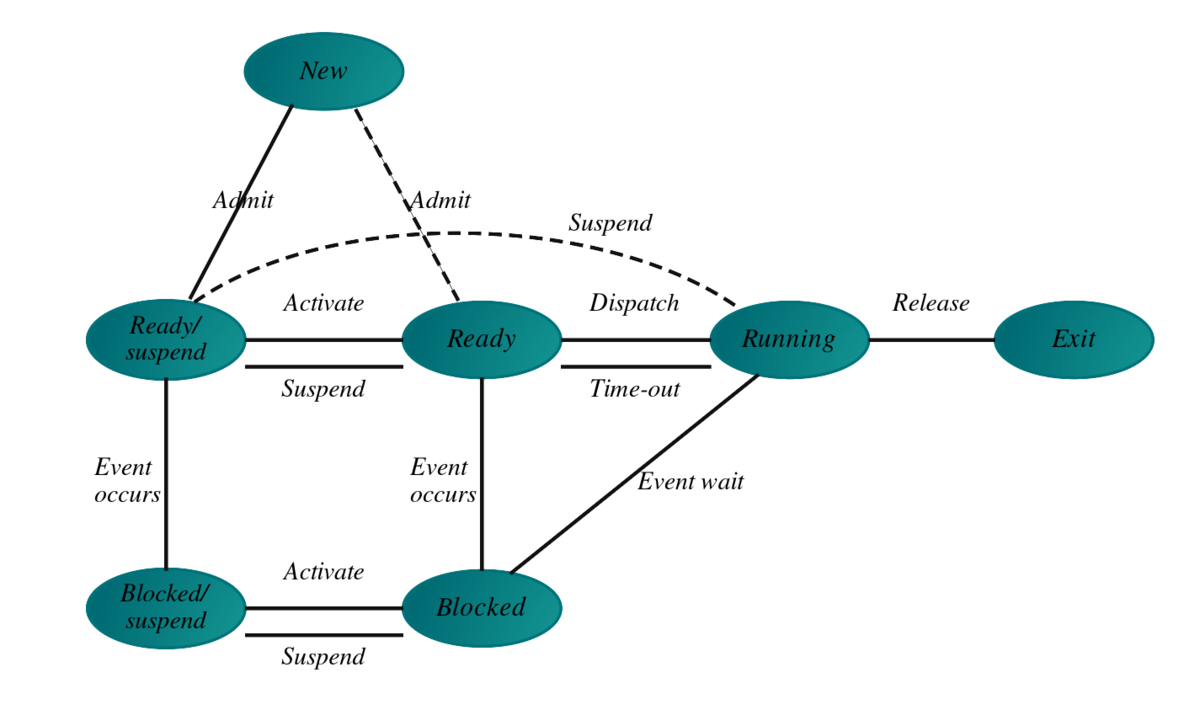
\includegraphics[width=\linewidth]{chapter3-seven-state.png}

\cheatsubsection{Control, Modes, Switching}
\term{Creation steps}: assign PID; allocate process space; initialize PCB; link into ready or suspend queues; create/expand accounting and other tables.\\
\term{User mode}: low privilege; cannot execute privileged instructions. \term{Kernel/System mode}: high privilege for protected OS operations.\\
\term{Interrupt}: asynchronous external event. \term{Trap}: exception caused by the current instruction. \term{Supervisor call}: explicit request for an OS service.\\
\term{Mode switch}: changes privilege mode, possibly same process. \term{Process switch}: CPU changes from one process to another.\\
\term{Process switch work}: save old PC, PSW, registers into PCB; update state and queues; choose next process; load next PCB/context.

\cheatsection{Chapter 3 Review Q\&A}
\begin{stemlist}
\stemrow{R3.1 Trace}{Stem: instruction trace. A: executed instruction sequence of a process.}
\stemrow{R3.2 Creation}{Stem: process creation events. A: new batch job, interactive logon, OS-created service, spawned child.}
\stemrow{R3.3 States}{Stem: Fig. 3.6 states. A: New, Ready, Running, Blocked, Exit.}
\stemrow{R3.4 Preempt}{Stem: preempt a process. A: reclaim CPU before the process voluntarily yields or finishes.}
\stemrow{R3.5 Swapping}{Stem: swapping and purpose. A: move process memory to/from disk to free memory and improve CPU use.}
\stemrow{R3.6 Two blocked}{Stem: why Fig. 3.9b has two blocked states. A: resident Blocked vs swapped-out Blocked/Suspend.}
\stemrow{R3.7 Suspended}{Stem: four suspended-process traits. A: not executable now; may wait; agent-suspended; explicitly activated.}
\stemrow{R3.8 OS tables}{Stem: OS management tables. A: memory, I/O, file, process.}
\stemrow{R3.9 PCB info}{Stem: three PCB categories. A: identification, processor state, process control.}
\stemrow{R3.10 Modes}{Stem: why user/kernel modes. A: protect OS, PCBs, memory, I/O, privileged instructions.}
\stemrow{R3.11 Create}{Stem: OS steps to create process. A: PID, space, PCB, links, other tables.}
\stemrow{R3.12 Int/trap}{Stem: interrupt vs trap. A: external asynchronous event vs instruction-caused exception.}
\stemrow{R3.13 Examples}{Stem: three interrupts. A: clock, I/O, memory fault.}
\stemrow{R3.14 Switches}{Stem: mode switch vs process switch. A: privilege change vs changing the running process.}
\end{stemlist}

\cheatsection{Chapter 3 Problem Q\&A}
\begin{stemlist}
\stemrow{P3.1 Transitions}{Stem: R/RUN/B/NR transition table. A: 1 dispatch; 2 preempt; 3 event wait; 4 event occurs; 5 ready swap-out; 6 blocked swap-out.}
\stemrow{P3.2 Timeline}{Stem: process states at \(t=22,37,47\). A: \(t=22\): P1 B(d3 read), P3 B(d2 read), P7 B(d3 write), P5 likely running. \(t=37\): P1/P3 ready, P5 Blocked/Suspend, P7 blocked, P8 running. \(t=47\): P5 ready, P7 blocked, P8 exit; one ready process may run.}
\stemrow{P3.3 Seven states}{Stem: possible/impossible Fig. 3.9b transitions. A: Possible direct moves: N\(\to\)R/RS/E; R\(\to\)Run/RS/E; Run\(\to\)R/B/RS/E; B\(\to\)R/BS/E; RS\(\to\)R/E; BS\(\to\)B/RS/E; all other direct moves are impossible.}
\stemrow{P3.4 Queues}{Stem: seven-state queueing diagram. A: Ready queue, processor, per-event Blocked queues, Ready/Suspend queue, and per-event Blocked/Suspend queues.}
\stemrow{P3.5 Policy}{Stem: choose Ready vs high-priority Ready/Suspend. A: swap in Ready/Suspend only when priority or aging benefit exceeds swap cost; otherwise dispatch resident Ready.}
\stemrow{P3.6 VAX states}{Stem: justify VAX/VMS wait states. A: many waits give precise event/resource queues; paging/global resource waits need no resident/outswapped pair; transitions follow dispatch, wait, event, swap.}
\stemrow{P3.7 Access modes}{Stem: four access modes vs two. A: Kernel, Executive, Supervisor, User give finer least-privilege protection, but add complexity and mode-switch overhead.}
\stemrow{P3.8 Rings}{Stem: ring protection need-to-know problem. A: rings are nested; inner domains can access outer objects, so selective need-to-know access is hard to enforce.}
\stemrow{P3.9 Multi-wait}{Stem: process waiting on multiple events. A: yes, e.g., network, keyboard, timeout; use wait descriptors or multiple queue links and remove stale links after wakeup.}
\stemrow{P3.10 Fixed saves}{Stem: fixed interrupt register-save locations. A: practical only for simple nonnested systems; nested interrupts, multiprogramming, and switches need PCB/kernel-stack context.}
\stemrow{P3.11 Real-time}{Stem: nonpreemptive kernel and real-time. A: it can cause unbounded latency, priority inversion, and missed deadlines; real-time systems need bounded response.}
\stemrow{P3.12 Fork}{Stem: possible output of successful \code{fork()}. A: two lines print: \(0\) in the child and child PID in the parent; order is scheduler-dependent.}
\end{stemlist}

\cheatsection{Chapter 3 Fast Recall}
\begin{itemize}
  \item Process = program in execution; PCB makes pause/resume possible.
  \item Ready lacks CPU; Blocked lacks an event; Suspended is out of main memory.
  \item Preemption takes CPU from a process before it yields.
  \item Interrupts are external; traps are instruction-caused; supervisor calls request OS services.
  \item A mode switch can stay in the same process; a process switch always changes processes.
  \item Context switching saves old PCB state and restores the selected process state.
\end{itemize}



\cheatsection{4 Threads}
\cheatsubsection{Process vs Thread}
\term{Process}: unit of resource ownership and protection; owns address space, process image, open files, I/O resources, privileges, and IPC links.\\
\term{Thread}: unit of scheduling/execution; has state, PC, registers, stack, priority, context, and thread-local data. Threads in one process share memory and resources.\\
\term{Multithreading}: multiple concurrent execution paths inside one process. \term{PCB} stores process resources; \term{TCB} stores thread execution context.\\
\term{Advantages}: faster create/terminate/switch, cheaper communication, better responsiveness, overlapped I/O and computation, true parallelism on multiprocessors.

\cheatsubsection{States, Operations, Synchronization}
\term{Thread states}: Running, Ready, Blocked. Suspend states are usually process-level because all threads share the process address space.\\
\term{Operations}: spawn creates a ready thread; block waits for an event; unblock moves to Ready; finish releases context and stack.\\
\term{Synchronization}: required because shared address space/resources can cause data races, lost updates, and corrupted data structures.

\cheatsubsection{ULT, KLT, Combined}
\term{ULT}: managed by a user-level thread library; kernel sees only the process. Pros: no kernel-mode switch, application scheduling, portable. Cons: blocking syscall may block all process threads; pure ULT cannot exploit multiprocessing.\\
\term{KLT}: managed and scheduled by the kernel. Pros: one blocked thread need not block the process; threads can run on multiple CPUs; kernel code can be multithreaded. Cons: higher switch overhead.\\
\term{Jacketing}: wrap a blocking system call so the thread library can test/yield and avoid blocking the whole process.\\
\term{Combined}: map many ULTs onto some KLTs/LWPs to mix fast user-level management with kernel parallelism.

\cheatsection{Chapter 4 Review Q\&A}
\begin{stemlist}
\stemrow{R4.1 PCB/TCB}{Stem: which PCB elements move to TCB. A: TCB gets thread state, PC, registers, stack pointer, priority, scheduling info, private data; PCB keeps PID, address space, memory, files/I/O, privileges, IPC.}
\stemrow{R4.2 Switch cost}{Stem: why thread mode switch may be cheaper. A: same-process threads keep the same address space and resources; only thread context is saved/restored.}
\stemrow{R4.3 Process traits}{Stem: two independent process characteristics. A: resource ownership and scheduling/execution.}
\stemrow{R4.4 Uses}{Stem: four thread uses. A: foreground/background work, asynchronous processing, faster execution by overlap/parallelism, modular program structure.}
\stemrow{R4.5 Shared resources}{Stem: resources shared by process threads. A: address space, code, global data, heap, files, I/O resources, privileges; each thread has own PC, registers, stack, state.}
\stemrow{R4.6 ULT pros}{Stem: three ULT advantages over KLTs. A: no kernel switch for thread ops, application-specific scheduling, portability.}
\stemrow{R4.7 ULT cons}{Stem: two ULT disadvantages. A: blocking syscall may block the whole process; pure ULT cannot use multiple CPUs in parallel.}
\stemrow{R4.8 Jacketing}{Stem: define jacketing. A: wrapper turns a blocking syscall into nonblocking behavior for user-level thread scheduling.}
\end{stemlist}

\cheatsection{Chapter 4 Problem Q\&A}
\begin{stemlist}
\stemrow{P4.1 Same-process switch}{Stem: same-process vs different-process thread switch. A: yes; same-process switch avoids address-space/resource switch.}
\stemrow{P4.2 ULT blocking}{Stem: why one blocking ULT blocks all. A: kernel is unaware of ULTs and blocks the whole process on a blocking syscall.}
\stemrow{P4.3 OS/2 sessions}{Stem: remove sessions, bind UI to processes. A: lose grouping of several processes under one UI; assign memory/files/resources to processes, not threads.}
\stemrow{P4.4 1:1 on uniprocessor}{Stem: why faster than single thread. A: when one thread waits for I/O, another ready thread can run; CPU use and responsiveness improve.}
\stemrow{P4.5 Process exit}{Stem: process exits while threads run. A: no thread continues; threads depend on the process address space/resources.}
\stemrow{P4.6 OS/390 ASCB/TCB}{Stem: split global ASCB and local TCB. A: separates address-space management from task execution and reduces global kernel data.}
\stemrow{P4.7 count\_positives}{Stem: function and two-thread risk. A: counts positive list values into a global counter; unsynchronized shared counter creates data-race risk.}
\stemrow{P4.8 Optimized code}{Stem: compiler caches global counter. A: local-register copy can overwrite another thread update, causing lost update.}
\stemrow{P4.9 Pthreads}{Stem: two threads increment \code{myglobal}; output 21. A: unexpected race; read-add-write is not atomic, so increments are lost.}
\stemrow{P4.10 Solaris yield}{Stem: yield to same priority only. A: a higher-priority runnable thread would normally be selected by the scheduler; yield donates only among equal-priority peers.}
\stemrow{P4.11 Solaris ULT/LWP}{Stem: many ULTs per LWP and state diagrams. A: fewer LWPs reduce kernel overhead; ULT state and LWP state differ because user library and kernel schedule different entities.}
\stemrow{P4.12 Linux uninterruptible}{Stem: rationale for Uninterruptible state. A: protect kernel/device consistency while waiting for critical I/O/resource events; wake only when event completes.}
\end{stemlist}

\cheatsection{Chapter 4 Fast Recall}
\begin{itemize}
  \item Process owns resources; thread executes code.
  \item Threads share process memory/resources but keep private PC, registers, stack, and state.
  \item ULT is fast and portable but weak on blocking and multiprocessing.
  \item KLT costs more but supports kernel scheduling, blocking isolation, and CPU parallelism.
  \item Race condition = unsynchronized shared read/write; lost update is the classic symptom.
\end{itemize}

\cheatsection{5 Concurrency and Semaphores}
\cheatsubsection{Concurrency Basics}
\term{Concurrency}: multiple processes or threads make progress in the same time interval. On one CPU execution is interleaved; on many CPUs it may overlap in parallel.\\
\term{Main hazards}: shared global resources, hard resource allocation, and nondeterministic bugs.\\
\term{Race condition}: final result depends on timing of unsynchronized shared read/write.\\
\term{Critical section}: code that accesses a shared resource. \term{Mutual exclusion}: at most one process may execute the corresponding critical section for the same resource.

\cheatsubsection{Interaction and OS Concerns}
\begin{tabularx}{\linewidth}{@{}lY@{}}
\toprule
\term{Unaware} & competition; issues: mutual exclusion, deadlock, starvation.\\
\term{Indirectly aware} & cooperation by sharing; add data coherence risk.\\
\term{Directly aware} & cooperation by communication; no shared-data mutex, but deadlock/starvation still possible.\\
\bottomrule
\end{tabularx}
\term{OS duties}: track processes, allocate/deallocate resources, protect data/resources, and ensure speed independence.

\cheatsubsection{Mutual Exclusion Requirements}
\begin{itemize}
  \item Only one process in a critical section for a resource.
  \item A halted noncritical process must not block others.
  \item No deadlock or starvation.
  \item If the critical section is free, entry is not delayed.
  \item Assume no process speed or processor count.
  \item A process stays in the critical section only finite time.
\end{itemize}

\cheatsubsection{Semaphores}
\term{Semaphore}: integer synchronization variable accessed only by atomic operations: initialize, \code{semWait}/P/down, \code{semSignal}/V/up.\\
\term{Count meaning}: \(s>0\) means available units; \(s=0\) means none free; \(s<0\) means \(|s|\) blocked waiters.\\
\term{Binary semaphore}: value 0/1, often mutex-like. \term{General/counting semaphore}: integer count for multiple resources or ordering.\\
\term{Mutex vs binary semaphore}: a mutex is unlocked by its locker; a binary semaphore may be waited by one process and signaled by another.\\
\term{Strong semaphore}: FIFO wait queue. \term{Weak semaphore}: no specified release order; starvation is possible.\\
\term{Implementation}: \code{semWait} and \code{semSignal} must be atomic; use hardware support, compare-and-swap, short interrupt disable on uniprocessors, or software algorithms.

\cheatsubsection{Producer/Consumer Patterns}
\term{Infinite buffer}: \code{n=0} counts items; \code{s=1} protects the buffer. Producer: wait \(s\), append, signal \(s\), signal \(n\). Consumer: wait \(n\), wait \(s\), take, signal \(s\).\\
\term{Bounded buffer}: \code{e=sizeofbuffer}, \code{n=0}, \code{s=1}. Producer: wait \(e\), wait \(s\), append, signal \(s\), signal \(n\). Consumer: wait \(n\), wait \(s\), take, signal \(s\), signal \(e\).\\
\note{Never wait on the resource count while holding the buffer mutex: producer wait \(s\) then \(e\), or consumer wait \(s\) then \(n\), can deadlock.}

\cheatsection{Chapter 5 Review Q\&A}
\begin{stemlist}
\stemrow{R5.1 Design issues}{Stem: four concurrency design issues. A: process communication, resource sharing/competition, synchronization, processor-time allocation.}
\stemrow{R5.2 Contexts}{Stem: three contexts where concurrency arises. A: multiple applications, structured applications, OS structure.}
\stemrow{R5.3 Basic requirement}{Stem: requirement for concurrent execution. A: enforce mutual exclusion for critical resources, with correct synchronization.}
\stemrow{R5.4 Awareness}{Stem: three degrees of process awareness. A: unaware/competition; indirectly aware/cooperation by sharing; directly aware/cooperation by communication.}
\stemrow{R5.5 Compete vs cooperate}{Stem: distinction. A: competing processes only contend for resources; cooperating processes work together by shared data or messages.}
\stemrow{R5.6 Control problems}{Stem: three competing-process problems. A: mutual exclusion, deadlock, starvation.}
\stemrow{R5.7 Mutex requirements}{Stem: list requirements. A: one-at-a-time, noncritical halt harmless, no deadlock/starvation, no needless delay, no speed/CPU assumptions, finite CS time.}
\stemrow{R5.8 Semaphore ops}{Stem: operations. A: initialize, \code{semWait}/P, \code{semSignal}/V; no direct arbitrary access.}
\stemrow{R5.9 Binary/general}{Stem: difference. A: binary is 0/1; general/counting is integer-valued for multiple units or synchronization.}
\stemrow{R5.10 Strong/weak}{Stem: difference. A: strong uses FIFO waiter release; weak gives no release-order guarantee.}
\stemrow{R5.11 Monitor}{Stem: monitor. A: high-level synchronization module encapsulating shared data/procedures; only one process active inside, with condition variables for waiting.}
\stemrow{R5.12 Messages}{Stem: blocking vs nonblocking. A: blocking send/receive waits for completion or message; nonblocking returns immediately after queueing or status check.}
\stemrow{R5.13 Readers/writers}{Stem: conditions. A: many readers may read together; writers need exclusive access; policies must avoid reader or writer starvation.}
\end{stemlist}

\cheatsection{Chapter 5 Problem Q\&A}
\begin{stemlist}
\stemrow{P5.1 Multi vs multiprocessing}{Stem: two concurrency differences. A: multiprogramming interleaves one CPU and can protect short regions by disabling interrupts; multiprocessing has true overlap, so one-CPU interrupt disable is insufficient.}
\stemrow{P5.3 Race traces}{Stem: print \code{x is 10} or \code{x is 8}. A: interleave the \code{if} test and \code{printf} to print 10; split load/decrement/store and load/increment/store to overwrite with stale 8.}
\stemrow{P5.4 Tally bounds}{Stem: two \code{total()} processes, \(n=50\). A: final \code{tally} is 2 to 100; with \(k\) processes, upper \(50k\), lower can still be 2 for \(k\ge2\).}
\stemrow{P5.5 Busy wait}{Stem: always less efficient than blocking? A: no; short waits may be cheaper than block/context-switch/restart overhead; long waits should block.}
\stemrow{P5.12 Sem definitions}{Stem: negative-count vs nonnegative-count semaphore definitions. A: equivalent to programs because waiters are represented either by negative count or by the queue; users cannot inspect internals.}
\stemrow{P5.16 General via binary}{Stem: flaw and fix. A: binary \code{delay} can lose wakeups; use pass-the-baton: if \code{semSignal} wakes a waiter, it signals \code{delay} instead of releasing \code{mutex}; awakened waiter releases \code{mutex}.}
\stemrow{P5.19 Consumer deadlock}{Stem: move empty-test inside mutex. A: consumer can hold \(s\) while waiting on \code{delay}; producer then waits for \(s\), so both block.}
\stemrow{P5.20 Faster infinite buffer}{Stem: reduce semaphore overhead. A: let \(n=-1\) mean empty and consumer waiting; producer signals \code{delay} only when append changes \(n\) from -1 to 0.}
\stemrow{P5.21 Swap order}{Stem: bounded-buffer statement swaps. A: swapping wait \(e/s\) or wait \(n/s\) can deadlock; swapping signal \(s/n\) or signal \(s/e\) preserves correctness but may add waiting.}
\stemrow{P5.22 Trace table}{Stem: fill bounded-buffer chart. A: blank labels: Pa p2, Pb p2, Pb p3, Cb c2, Pc p2, Cb c3, Pa p3, Pc p3, Pa p2, Pa p3; use FIFO queues; final state full \(=3\), empty \(=0\), buffer \(=XXX\).}
\end{stemlist}

\cheatsection{Chapter 5 Fast Recall}
\begin{itemize}
  \item Race condition = timing-dependent result on shared data.
  \item Protect the code that touches shared state, not just the variable name.
  \item P/down may block; V/up may wake zero or one waiter.
  \item Semaphore waits before mutex waits in producer/consumer resource tests.
  \item Strong semaphore fairness comes from FIFO; weak semaphore may starve.
\end{itemize}

\end{multicols*}

\end{document}
